%
% This is Chapter 1 file (chap1.tex)
%
\chapter{UX Quality Assurance}
A design evaluation for the final project of CISC472, evaluating the groupproject of Cong Meng and Owen Li. Hosted versions of the project can be foundat diy-reddit-257012.web.app and at https://github.com/udcymen/diy-reddit.

\section{Overview}

Below is a screenshot of the home page. Ignoring post content, which is understandably meaningless because of numerous test posts, we can still see several flaws.
\\\\
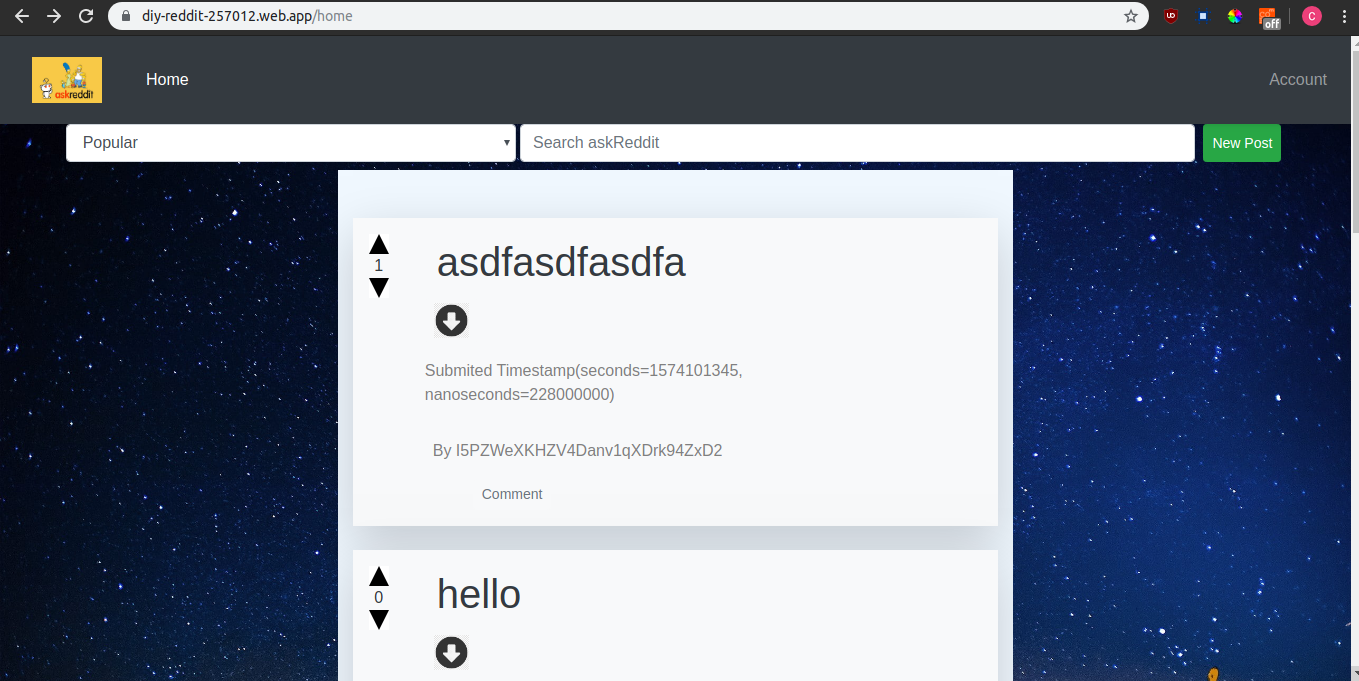
\includegraphics[width = 400pt]{images/home.png}
\begin{itemize}
    \item There is an incredible volume of useless or confusing information. Timestamps are given in nanoseconds and seconds, but not as dates or another, more easily consumable format.
    \item Posts are not ordered correctly by genre or other filters. Furthermore, the 'subreddit' chooser does nothing. The dropdown isn't the most user-friendly choice, and any tab shows the exact same posts, and fails to show more than about 10. After this, no new posts can be seen. Even posts with negative votes appear above many of those with positive counts.
    \item When creating a new post, you are given a rather well designed popup that alerts you of the post ID (a link or simple alert without a long id string might have been better). However, as previously mentioned, there is no way to see this post. Additionally, navigating to the Account page does not correctly list posts.
    \item Navigating between pages feels jittery. Rather than waiting to render the page until a response has been received, the page renders, and then it is populated after post data is received from the backend.
    \item There is little consistency in design. Default fonts are used sporadically, with confusing mixes of serif and sans-serif. The logo and background contain characters from The Simpsons.
    \item The Account Page has some useless buttons (see below), While the buttons are well styled, they are inconsistent (see the plaintext home link and the well-styled Sign Out Button).
\end{itemize}
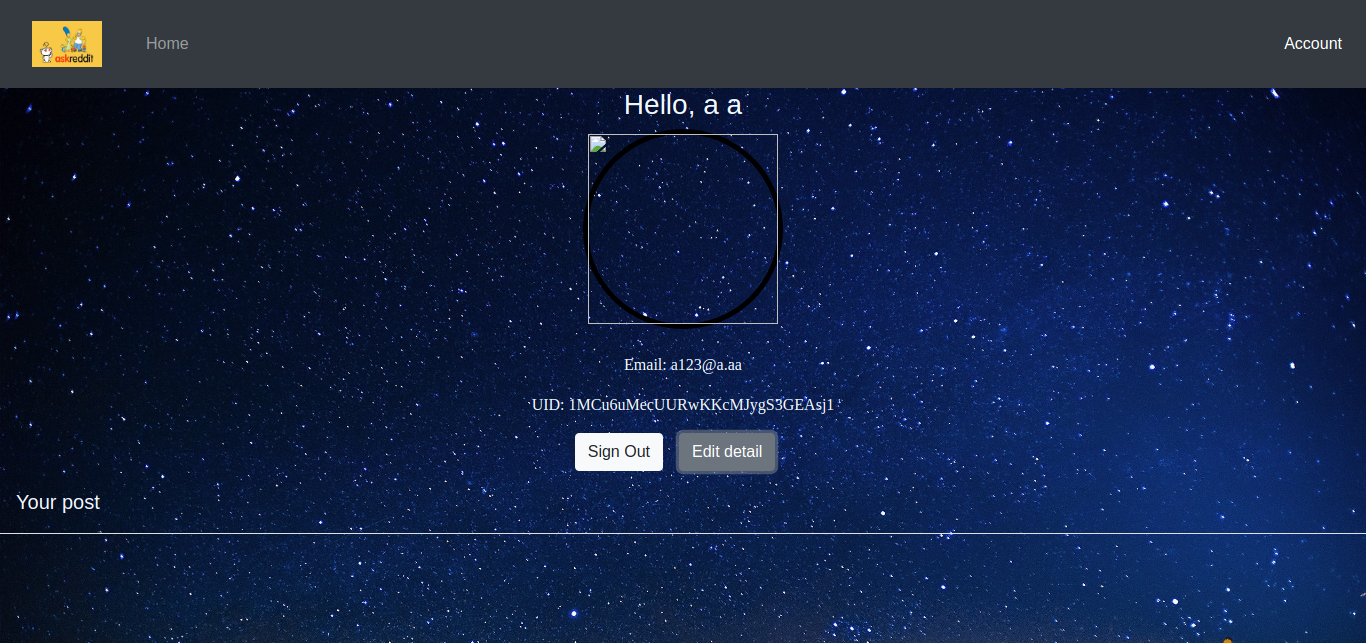
\includegraphics[width = 400pt]{images/account.png}
\begin{itemize}
    \item The forgot password button does not work.
    \item The individual post view is much better, as it shows comment dates. However, it still displays poster IDs, which is also a pontential security concern. Additionally, the content is prefixed by the words 'Content' in the exact same font as the content, which is unneccesary and confusing.
    \item I found some elements to be too large. Even though my laptop screen is 1376*768px, it still felt like I was browsing on a mobile phone.
    \item The mobile version of the site is not functional. Buttons are hidden and the site is not entirely responsive.
\end{itemize}

Put simply, this project feels unfinished. understandably, it will not be fully featured, but it should be expected that features present should be fully fleshed out.

\section{Evaluation}

The website as it stands is still fairly simple, but it is almost functional enough for a production environment from a UX perspective. The single largest shortcoming is the inability to see new posts. After than, it is the useless functionality of the subreddit selector. Fixing these elements would effectively make the product MVP-ready.

\section{Suggestions}
Spending an hour cleaning up vestigal controls, make all styling uniform, and fixing spacing, sizing, and overflow rules would solve 50\% of issues. Additionally, the issues with timestamps being displayed in nanoseconds should be a simple fix, considering it was done correctly in other areas of the site. Removing IDs and replacing them with a username would also be a good idea.

The remainder of shortcomings result from unexpected behavior. Adding tags to posts that allow the subreddit selector to correctly filter would add tremendous amount of depth to the user experience. Fixing the inability to see new posts, and incorrect sorting of posts based on votes would also fix most of the user experience.

Finally, adding more to the site in general would be useful: Descriptions, a solid background (the current background is distracting), and sidebars, would drive  user interaction and reduce the feeling of an 'empty' application.